\documentclass[landscape,final,a0paper]{../baposter}


\tracingstats=2

\usepackage{url}
\usepackage{calc}
\usepackage{graphicx}
\usepackage{amsmath}
\usepackage{amssymb}
\usepackage{relsize}
\usepackage{multirow}
\usepackage{bm}
\usepackage{tcolorbox}

\usepackage{graphicx}
\graphicspath{ {../img/} } 


\usepackage{multicol}

\usepackage{pgfbaselayers}
\pgfdeclarelayer{background}
\pgfdeclarelayer{foreground}
\pgfsetlayers{background,main,foreground}



% lmodern
\usepackage{lmodern}
\renewcommand{\familydefault}{\sfdefault}

% Comment out Helvetica
% \usepackage{helvet}
\usepackage{times}
\usepackage{palatino}

%\usepackage{tgbonum}

\newcommand{\captionfont}{\footnotesize}

\selectcolormodel{cmyk}

%\graphicspath{{images/}}

%%%%%%%%%%%%%%%%%%%%%%%%%%%%%%%%%%%%%%%%%%%%%%%%%%%%%%%%%%%%%%%%%%%%%%%%%%%%%%%%
%%%% Some math symbols used in the text
%%%%%%%%%%%%%%%%%%%%%%%%%%%%%%%%%%%%%%%%%%%%%%%%%%%%%%%%%%%%%%%%%%%%%%%%%%%%%%%%
% Format 

\renewcommand{\Pr}{\mbox{P}}
\newcommand{\e}{\mbox{e}}
\newcommand{\dx}{\,\mbox{d}x}

%%%%%%%%%%%%%%%%%%%%%%%%%%%%%%%%%%%%%%%%%%%%%%%%%%%%%%%%%%%%%%%%%%%%%%%%%%%%%%%%
% Multicol Settings
%%%%%%%%%%%%%%%%%%%%%%%%%%%%%%%%%%%%%%%%%%%%%%%%%%%%%%%%%%%%%%%%%%%%%%%%%%%%%%%%
\setlength{\columnsep}{0.7em}
\setlength{\columnseprule}{0mm}


%%%%%%%%%%%%%%%%%%%%%%%%%%%%%%%%%%%%%%%%%%%%%%%%%%%%%%%%%%%%%%%%%%%%%%%%%%%%%%%%
% Save space in lists. Use this after the opening of the list
%%%%%%%%%%%%%%%%%%%%%%%%%%%%%%%%%%%%%%%%%%%%%%%%%%%%%%%%%%%%%%%%%%%%%%%%%%%%%%%%
\newcommand{\compresslist}{%
\setlength{\itemsep}{1pt}%
\setlength{\parskip}{0pt}%
\setlength{\parsep}{0pt}%
}


%%%%%%%%%%%%%%%%%%%%%%%%%%%%%%%%%%%%%%%%%%%%%%%%%%%%%%%%%%%%%%%%%%%%%%%%%%%%%%
%%% Begin of Document
%%%%%%%%%%%%%%%%%%%%%%%%%%%%%%%%%%%%%%%%%%%%%%%%%%%%%%%%%%%%%%%%%%%%%%%%%%%%%%

\begin{document}

%%%%%%%%%%%%%%%%%%%%%%%%%%%%%%%%%%%%%%%%%%%%%%%%%%%%%%%%%%%%%%%%%%%%%%%%%%%%%%
%%% Here starts the poster
%%%---------------------------------------------------------------------------
%%% Format it to your taste with the options
%%%%%%%%%%%%%%%%%%%%%%%%%%%%%%%%%%%%%%%%%%%%%%%%%%%%%%%%%%%%%%%%%%%%%%%%%%%%%%
% Define some colors
\definecolor{silver}{cmyk}{0,0,0,0.3}
\definecolor{yellow}{cmyk}{0,0,0.9,0.0}
\definecolor{reddishyellow}{cmyk}{0,0.22,1.0,0.0}
\definecolor{black}{cmyk}{0,0,0.0,1.0}
\definecolor{darkYellow}{cmyk}{0,0,1.0,0.5}
\definecolor{darkSilver}{cmyk}{0,0,0,0.1}
\definecolor{lightyellow}{cmyk}{0,0,0.3,0.0}
\definecolor{lighteryellow}{cmyk}{0,0,0.1,0.0}
\definecolor{lighteryellow}{cmyk}{0,0,0.1,0.0}
\definecolor{lightestyellow}{cmyk}{0,0,0.05,0.0}
\definecolor{cyan}{cmyk}{1,0,0,0}
\definecolor{lightcyan}{cmyk}{0.5,0,0,0}
\definecolor{pastelcyan}{cmyk}{0.25,0,0,0}
\definecolor{magenta}{cmyk}{0,1,0,0}
\definecolor{yellow}{cmyk}{0,0,1,0}
\definecolor{lightyellow}{cmyk}{0,0,0.5,0}
\definecolor{pastelyellow}{cmyk}{0,0,0.25,0}
\definecolor{black}{cmyk}{0,0,0,1}
\definecolor{darkgray}{cmyk}{0,0,0,0.75}
\definecolor{gray}{cmyk}{0,0,0,0.5}
\definecolor{lightgray}{cmyk}{0,0,0,0.25}
\definecolor{white}{cmyk}{0,0,0,0}
\definecolor{red}{cmyk}{0,1,1,0}
\definecolor{orange}{cmyk}{0,0.5,1,0}
\definecolor{scarlet}{cmyk}{0,1,0.5,0}
\definecolor{brown}{cmyk}{0.5,0.75,1,0}
\definecolor{camel}{cmyk}{0.25,0.375,0.5,0}
\definecolor{cream}{cmyk}{0,0.2,0.3,0}
\definecolor{green}{cmyk}{1,0,1,0}
\definecolor{lightgreen}{cmyk}{0.5,0,0.5,0}
\definecolor{pastelgreen}{cmyk}{0.25,0,0.25,0}
\definecolor{mossgreen}{cmyk}{0.64,0.4,1,0}
\definecolor{yellowgreen}{cmyk}{0.5,0,1,0}
\definecolor{skyblue}{cmyk}{0.4,0.16,0,0}
\definecolor{royal}{cmyk}{1.0,0.5,0,0}
\definecolor{navyblue}{cmyk}{0.9,0.75,0.5,0}
\definecolor{lightnavy}{cmyk}{0.4,0.3,0.2,0}
\definecolor{blue}{cmyk}{1,1,0,0}
\definecolor{lightblue}{cmyk}{0.5,0.5,0,0}
\definecolor{pastelblue}{cmyk}{0.25,0.25,0,0}
\definecolor{lightpastelblue}{cmyk}{0.16,0.5,0,0.5}
\definecolor{lightestpastelblue}{cmyk}{0.05,0.05,0,0}
\definecolor{lavender}{cmyk}{0.25,0.25,0,0}
\definecolor{violet}{cmyk}{0.75,1,0.25,0}
\definecolor{purple}{cmyk}{0.5,1,0.5,0}
\definecolor{lightpurple}{cmyk}{0.25,0.5,0.25,0}
\definecolor{pink}{cmyk}{0,0.5,0,0}

\colorlet{HeaderBackground}{royal} % <-- added
\colorlet{PosterBackground}{white}  % <-- added

%%

\typeout{Poster Starts}
%\background{
  %\begin{tikzpicture}[remember picture,overlay]%
  %  \draw (current page.north west)+(-2em,-2em) node[anchor=north west] %{\hspace{-2em}\includegraphics[height=1.1\textheight]{silhouettes_background}};
 % \end{tikzpicture}%
%}


\background{
    \begin{tikzpicture}[remember picture,overlay]%
    %the poster background color
    \fill[fill=PosterBackground] (current page.north west) rectangle (current page.south east); %% cover the whole poster
    %the header
    \fill [fill=HeaderBackground] (current page.north west) rectangle ([yshift=-\headerheight] current page.north east); % just for the poster header, fill with a different color.
    \end{tikzpicture}
}

\newlength{\leftimgwidth}
\begin{poster}%
  % Poster Options, such as colours etc
  {
  % Show grid to help with alignment
  grid=false,
 % Column spacing
  colspacing=0.5em,
 % Color style
  bgColorOne=pink,
  bgColorTwo=red,
  borderColor=white,
  headerColorOne=royal,
  headerColorTwo=purple,
  headerFontColor=white,
  boxColorOne=white,
  boxColorTwo=green,
 % Format of textbox
  textborder=roundedleft,
% textborder=rectangle,
% Format of text header
  eyecatcher=true,
  headerborder=open,
  headerheight=0.10\textheight,
  headershape=smallrounded,
  headershade=plain,
  headerfont=\Large\sf\mdseries, 
  % headerfont=\Large\textsf, %Sans Serif
  boxshade=plain,
%  background=shade-tb,
 % background=plain,
  background=user,
  linewidth=2pt,
  %set the number of columns
  columns=12
  }
  % Eye Catcher
  {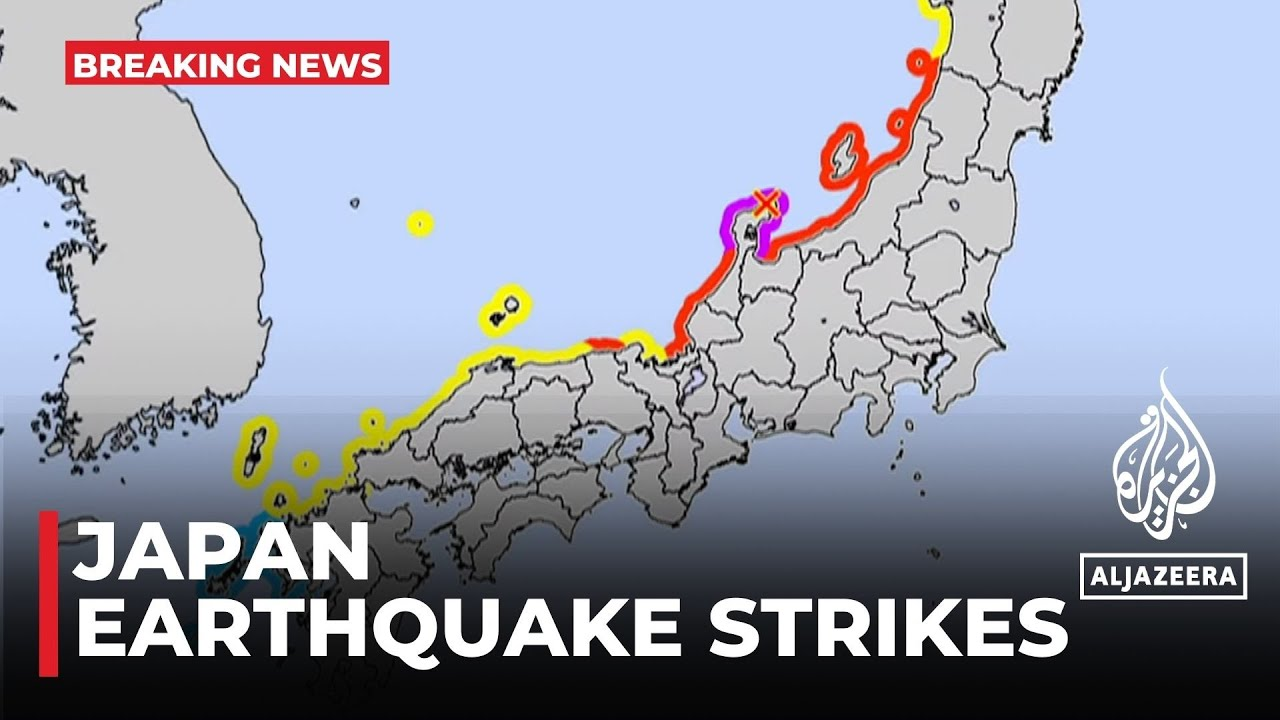
\includegraphics[width=10.5em]{Blackboard files/img/je.png}} % select eyecatcher=false above if not required. If no eye catcher is present, the title is left aligned.
  % Title
  {\sffamily\bfsereies\textcolor{white}{ %Sans Serif
  %\bf% Serif
   Seismographic Modelling via Hawkes Processes}}
  % Authors
  {\sf %Sans Serif
  % Serif
  \vspace{1em} 
	\textcolor{white}{David Ye \quad CID: 02395607 \quad dy1223@ic.ac.uk}\\
  }
  % University logo
  { % The makebox allows the title to flow into the logo
    \makebox[8em][r]{%
        \begin{minipage}{16em}
				\hfill 
\includegraphics[width=5cm]{Blackboard files/img/iclogo.png}
				\end{minipage}
      
    }
  }

  \tikzstyle{light shaded}=[top color=baposterBGtwo!30!white,bottom color=baposterBGone!30!white,shading=axis,shading angle=30]

  % Width of left inset image
     \setlength{\leftimgwidth}{0.78em+8.0em}

%%%%%%%%%%%%%%%%%%%%%%%%%%%%%%%%%%%%%%%%%%%%%%%%%%%%%%%%%%%%%%%%%%%%%%%%%%%%%%
%%% Now define the boxes that make up the poster
%%%---------------------------------------------------------------------------
%%% Each box has a name and can be placed absolutely or relatively.
%%% The only inconvenience is that you can only specify a relative position 
%%% towards an already declared box. So if you have a box attached to the 
%%% bottom, one to the top and a third one which should be in between, you 
%%% have to specify the top and bottom boxes before you specify the middle 
%%% box.
%%%%%%%%%%%%%%%%%%%%%%%%%%%%%%%%%%%%%%%%%%%%%%%%%%%%%%%%%%%%%%%%%%%%%%%%%%%%%%
    %
%     % A coloured circle useful as a bullet with an adjustably strong filling
% \newcommand{\colouredcircle}[1]{%
%       \tikz{\useasboundingbox (-0.2em,-0.32em) rectangle(0.2em,0.32em); \draw[draw=black,fill=baposterBGone!80!black!#1!white,line width=0.03em] (0,0) circle(0.18em);}}

%%%%%%%%%%%%%%%%%%%%%%%%%%%%%%%%%%%%%%%%%%%%%%%%%%%%%%%%%%%%%%%%%%%%%%%%%%%%%%
  \headerbox{Introduction}{name=intro,column=0,row=0, span = 3}{
%%%%%%%%%%%%%%%%%%%%%%%%%%%%%%%%%%%%%%%%%%%%%%%%%%%%%%%%%%%%%%%%%%%%%%%%%%%%%%
The Hawkes process is a type of stochastic point process characterized by self-exciting behavior, where the occurrence of an event increases the likelihood of subsequent events in the near future. This phenomenon is common in nature and has practical applications in seismology, finance, epidemiology...
 }

%%%%%%%%%%%%%%%%%%%%%%%%%%%%%%%%%%%%%%%%%%%%%%%%%%%%%%%%%%%%%%%%%%%%%%%%%%%%%%
  \headerbox{Definition}{name=defn,column=0,below=intro, span = 3}{
%%%%%%%%%%%%%%%%%%%%%%%%%%%%%%%%%%%%%%%%%%%%%%%%%%%%%%%%%%%%%%%%%%%%%%%%%%%%%%
    Let \(\{t_1, t_2, \ldots, t_k\}\) be the realizations of the past event arrival times, and let  $\lambda^*(t)$ denote the conditional intensity function that represents the instantaneous rate of event occurrence at time $t$, given the history of events $\mathcal{H}_t$ up to $t$.  $\lambda^*(t)$ of a Hawkes Process is then defined as:

\[
\lambda^*(t) = \lambda(t \mid \mathcal{H}_t) = \mu(t) + \sum_{t_i < t} \phi(t - t_i)
\]

where $\mu(t)$ is the background intensity and $\phi(t)$ is the excitation function (also known as the kernel). \\


For modelling seismic activity, we assume that the natural rate at which earthquakes occur is roughly constant, thus the background intensity $\mu(t) = \mu$ with  $\mu \in \mathbb{R}^+$ is chosen. We further assume that the time elapsed between each earthquake and an aftershock roughly follows an exponential distribution with decay rate $\beta$, thus the exponential kernel $\phi(t) = \alpha \beta e^{-\beta t}$ with $\alpha,\beta \in \mathbb{R}^+$ is chosen.


  }

%%%%%%%%%%%%%%%%%%%%%%%%%%%%%%%%%%%%%%%%%%%%%%%%%%%%%%%%%%%%%%%%%%%%%%%%%%%%%%
  \headerbox{Branching Ratio}{name=ratio,column=0,below=defn, above=foottext, span = 3}{

%%%%%%%%%%%%%%%%%%%%%%%%%%%%%%%%%%%%%%%%%%%%%%%%%%%%%%%%%%%%%%%%%%%%%%%%%%%%%%
For Hawkes Process with constant intensity, the branching ratio $\eta$ is defined as the expected number of events excited by a single event. Mathematically, it is written as:

\vspace{-1em}

\[
\eta = \int_{0}^{\infty} \phi(t) \, dt
\]

where $\phi(t)$ is the kernel of the Hawkes Process [2]. If $\eta < 1$, we say the Hawkes Process satisfies the stationarity condition. This can be understood by considering the expectation of $\lambda^*(t)$, where we have that $\mathbb{E}[\lambda^*(t)] = \frac{\mu}{1 - \eta}$, which is defined and positive if and only if  $\eta < 1$.\\

\vspace{-0.15em}

Note for the exponential kernel defined above, the branching ratio $\eta = \alpha$, which explains why the factorization of the constant is useful.



 }
 

%%%%%%%%%%%%%%%%%%%%%%%%%%%%%%%%%%%%%%%%%%%%%%%%%%%%%%%%%%%%%%%%%%%%%%%%%%%%%%
  \headerbox{Simulation}{name=simul,column=3,span=5, row=0}{

\vspace{-0.5em}
\begin{minipage}[t]{0.3\textwidth}
    \centering
    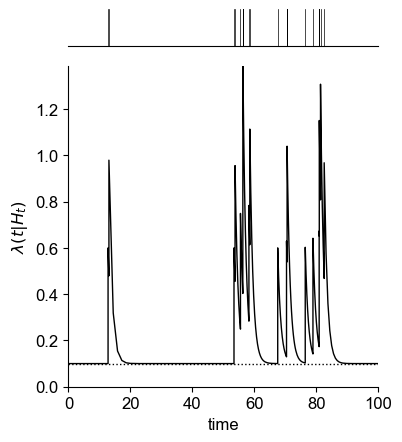
\includegraphics[width=\textwidth]{Blackboard files/img/Picture/Picture1.png}
    \captionof{$\mu = 0.1, \alpha = 0.5, \beta = 1.0$}
\end{minipage}
\hfill
\begin{minipage}[t]{0.3\textwidth}
    \centering
    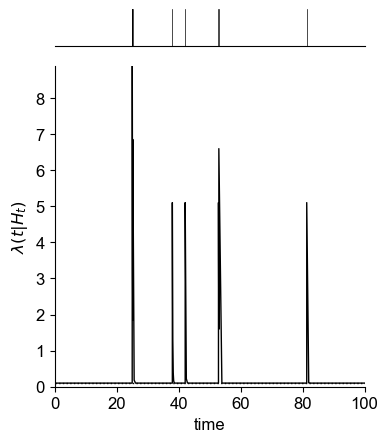
\includegraphics[width=\textwidth]{Blackboard files/img/Picture/Picture2.png}
    
    \captionof{$\mu = 0.1, \alpha = 0.5, \beta = 10.0$}
\end{minipage}
\hfill
\begin{minipage}[t]{0.3\textwidth}
    \centering
    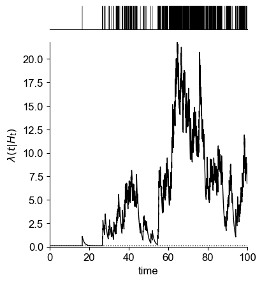
\includegraphics[width=\textwidth]{Blackboard files/img/Picture/Picture3.png}
    \captionof{$\mu = 0.1, \alpha = 1.0, \beta = 1.0$}
\end{minipage}


\vspace{0.5em}

As seen in the realizations, if $\alpha \geq 1$, the Hawkes Process does not satisfy the stationarity condition and $\lambda^*(t)$ becomes explosive, making it an unreliable model. For $\beta >> \alpha$, the decay times become more instantaneous and $\lambda^*(t)$ decays more rapidly after peaking, meaning for an average case one would expect less clustering.
	
  }
  



%%%%%%%%%%%%%%%%%%%%%%%%%%%%%%%%%%%%%%%%%%%%%%%%%%%%%%%%%%%%%%%%%%%%%%%%%%%%%%


\headerbox{Parameter Estimation}{name=esti,column=3,span=5,below=simul}{


\textbf{Theorem (Hawkes Process Likelihood [3])} Let \(N(\cdot)\) be a regular point process on \([0,T]\) for some finite positive \(T\), and let \(t_1, \ldots, t_k\) denote a realization of \(N(\cdot)\) over \([0,T]\). Then, the likelihood \(L\) of \(N(\cdot)\) is expressible in the form

\[
L = \left(\prod_{i=1}^k \lambda^*(t_i)\right) \exp \left(- \int_0^T \lambda^*(u) \, du\right).
\]


It then can be shown that if $\lambda^*(t)$ has a constant background intensity $\mu(t) = \mu$ and an exponential kernel $\phi(t) = \alpha \beta e^{-\beta (t)}$, then $L$ can be simplified and the log likelihood $l(\mu, \alpha, \beta)$ of $\lambda^*(t)$ is:

\[
l(\mu, \alpha, \beta) = \sum_{i=1}^k \log \left[ \mu + \alpha \sum_{j=1}^{i-1} e^{-\beta(t_i - t_j)} \right] - \mu t_k + {\alpha} \sum_{i=1}^k \left[ e^{-\beta(t_k - t_i)} - 1 \right].
\]

The log-likelihood is now expressed in terms of the 3 parameters, thus finding the parameters with maximum likelihood is now an optimization task that can be carried out systematically using calculus. \\

Applying this to the modelling of seismic activity, I used the USGS (United States Geological Survey) earthquake API to first collect earthquake data in Japan from 2023 January 1st to 2023 March 1st, with minimum magnitude set to 3.0. I then transformed the timestamps with 2023 January 1st 00:00 being 0 and unit being hours, and then used the list to estimate the parameters with maximum likelihood, which were calculated to be:

  \vspace{-2mm}
  \begin{center}
  $\mu \approx \textbf{0.09633} \quad \alpha \approx \textbf{0.09488} \quad \beta \approx \textbf{1.75153}$
  \end{center}

\vspace{-0.2em}

Interpreting the calculated parameters of this model: The natural rate of earthquakes occurrence is approximately 0.1, which implies one earthquake with magnitude over 3.0 occurs every $1/\mu \approx 10$ hours in Japan. Each earthquake results in $\alpha \approx 0.1$ aftershock on average, and aftershocks occur with $1/\beta \approx 0.57$ hours delay on average.


}

%%%%%%%%%%%%%%%%%%%%%%%%%%%%%%%%%%%%%%%%%%%%%%%%%%%%%%%%%%%%%%%%%%%%%%%%%%%%%%
  \headerbox{Evaluation}{name=eval,column=8,row=0, span = 2}{

 \vspace{0.5em}

    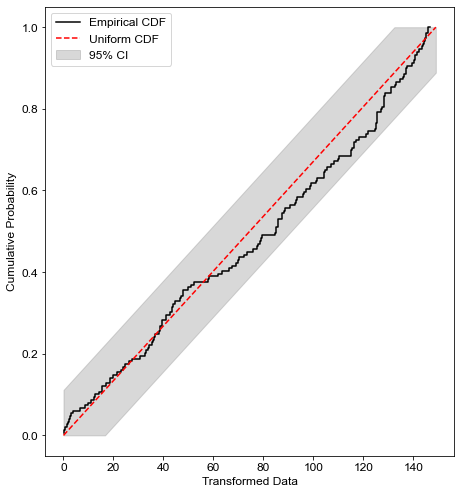
\includegraphics[width=\textwidth]{Blackboard files/img/test_final.png}

 \vspace{0.3em}


By the Time-Rescaling Theorem, we can test the accuracy of the model using the Kolmogorov-Smirov test, under the null hypothesis that the transformed times are uniformly distributed on the interval $[0, \Lambda(T)]$. The Empirical CDF of the transformed data is within the 95\% confidence interval of the uniform distribution, and the p-value is calculated to be approximately 0.102, which is greater than the common threshold of 0.05. From this, we fail to reject the null hypothesis.



  }


%%%%%%%%%%%%%%%%%%%%%%%%%%%%%%%%%%%%%%%%%%%%%%%%%%%%%%%%%%%%%%%%%%%%%%%%%%%%%%

\headerbox{Forecasting}{name=fc,column=10,row=0, span = 2}{


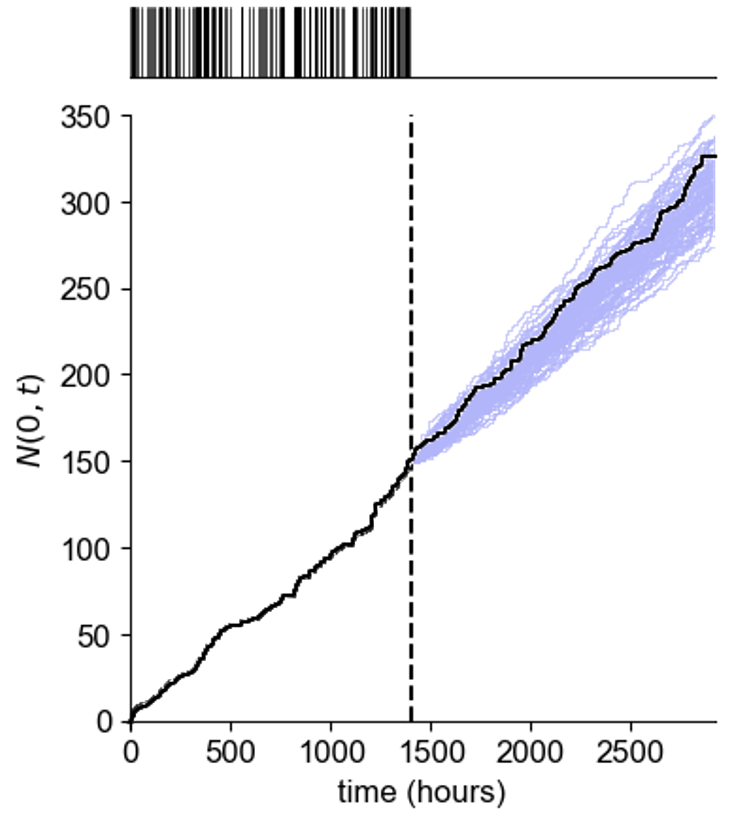
\includegraphics[width=\textwidth]{Blackboard files/img/Picture/Pred.png}

The black line represents the empirical counting process of earthquakes in Japan from 2023 January 1st to 2023 May 1st, and the blue lines represent 100 simulated realizations of the counting process using the estimated parameters, which are used to predict the counting process of earthquakes from 2023 March 1st to 2023 May 1st. The black line completely lies inside the bounds formed by the blue lines, which suggests the model has some level of forecasting power.

}


%%%%%%%%%%%%%%%%%%%%%%%%%%%%%%%%%%%%%%%%%%%%%%%%%%%%%%%%%%%%%%%%%%%%%%%%%%%%%%
\headerbox{Conclusions}{name=concl,column=8,below=fc, span = 4}{

In this study, I explored the theory of Hawkes Process and its application in real-life modeling. I collected seismic activity data from Japan and used it to construct a basic Hawkes Process model, which was then used to predict future earthquake trend in the region. \\ 
Although the model is an oversimplification, it illustrates the fundamental idea of how Hawkes Process is applied in seismology. The model can be further improved with more training data, choosing non-parametric approaches, or taking into account the location and magnitude of each earthquake through marked or multivariate Hawkes processes. These are all possible areas for further exploration.

	}
	
%%%%%%%%%%%%%%%%%%%%%%%%%%%%%%%%%%%%%%%%%%%%%%%%%%%%%%%%%%%%%%%%%%%%%%%%%%%%%%
  \headerbox{References}{name=references,column=8,above=bottom, span = 4}{
    \smaller
    \vspace{-0.4em}
    \bibliographystyle{plain}
    \renewcommand{\section}[2]{\vskip 0.05em}
      \begin{thebibliography}{1}\itemsep=-0.01em
      \setlength{\baselineskip}{0.4em}
      \bibitem{hawkes}
      Hawkes, A. G. Spectra of some self-exciting and mutually exciting point processes.
      \bibitem{branching}
      Hardiman, S. J. & Bouchaud, J. (2014) Branching ratio approximation for the self-exciting Hawkes process.
      \bibitem{daleyi}
      Daley, D. J. \& Vere-Jones, D. (2003) Introduction to the Theory of Point Processes, Volume I. Probability and Its Applications. 2nd edition. New York, NY, Springer.
      
      
      \end{thebibliography}
  }
%%%%%%%%%%%%%%%%%%%%%%%%%%%%%%%%%%%%%%%%%%%%%%%%%%%%%%%%%%%%%%%%%%%%%%%%%%%%%%



  
\end{poster}

\end{document}
